\begin{frame}{CDC検出効率}
  \label{page:effCDC}
  
  Run78でがIHがアンインストールされている \\
  Run68のデータでIHをトリガーとして使う
  \tminipageThree{
    \begin{figure}
      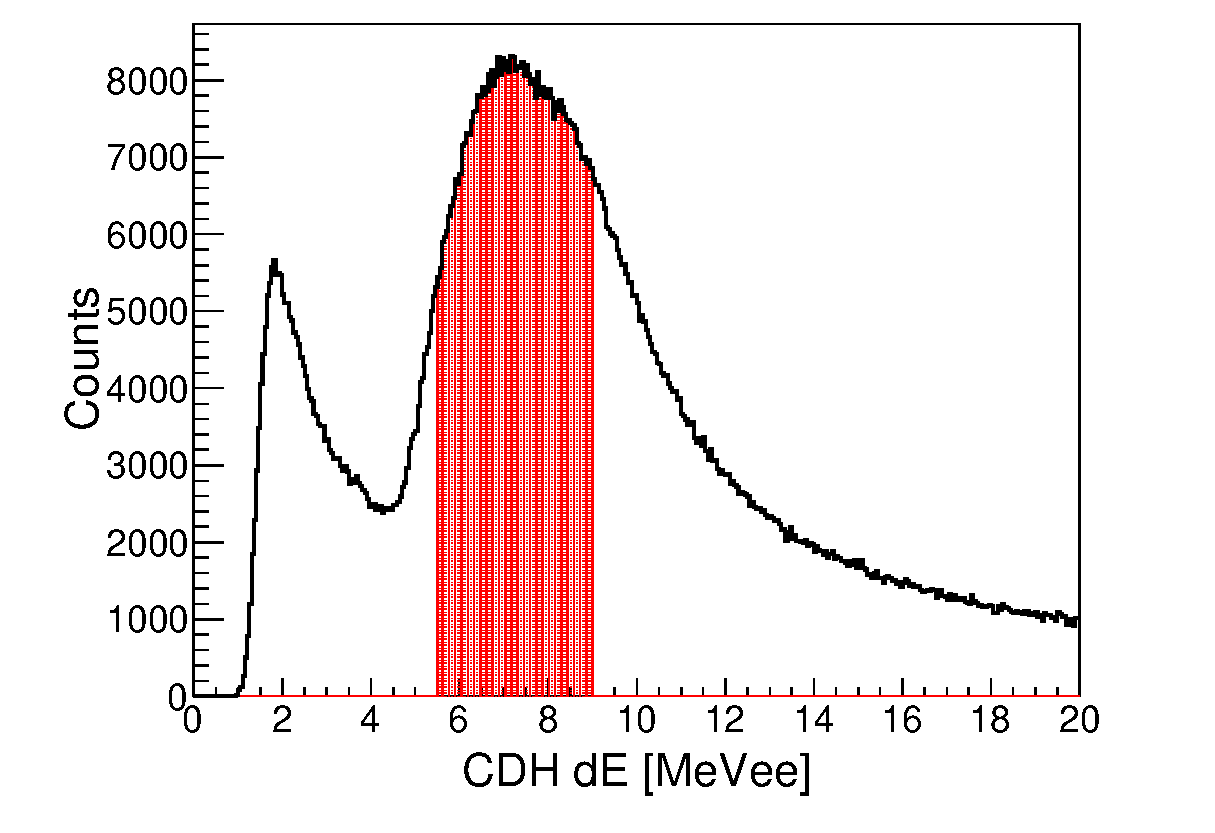
\includegraphics[width=3cm]{../pic/Run68/CDC_eff/CDH_dE.eps}
    \end{figure}
  }{
    \begin{figure}
      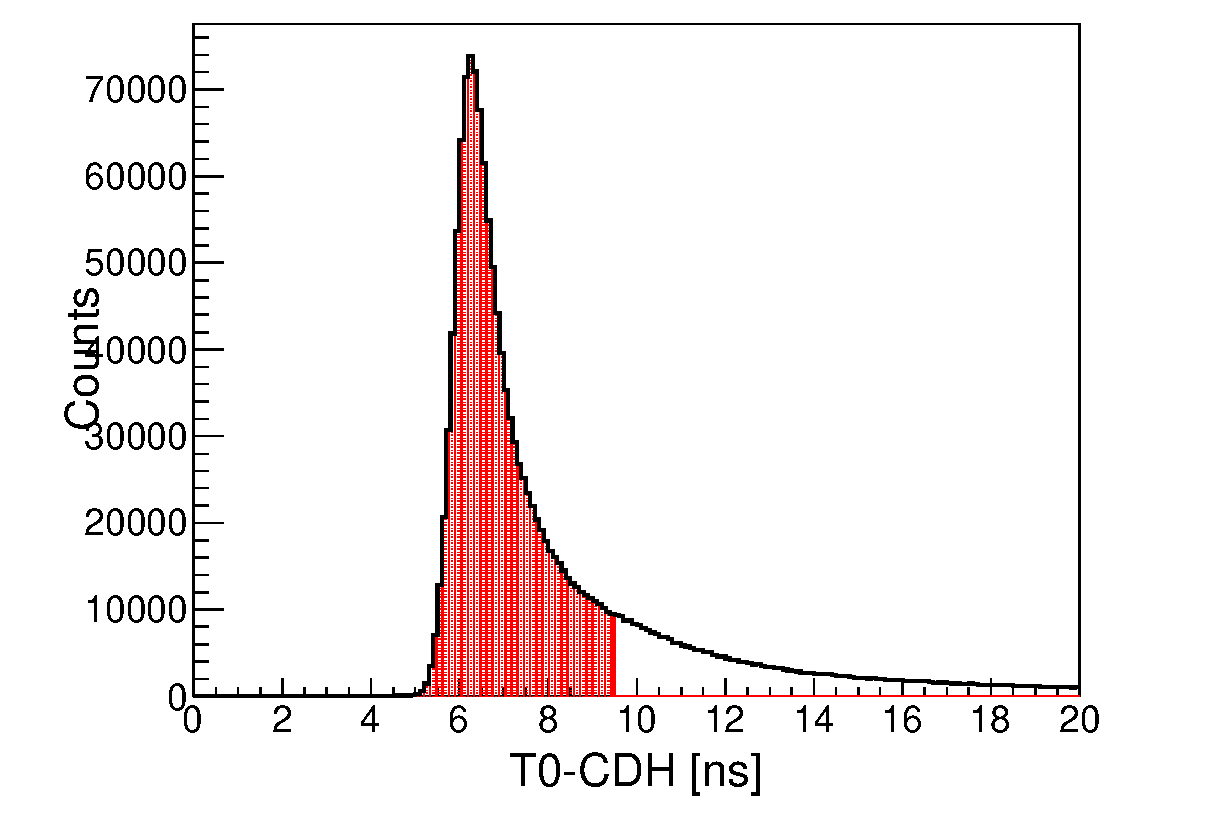
\includegraphics[width=3cm]{../pic/Run68/CDC_eff/CDH_tof.eps}
    \end{figure}
  }{
    \begin{figure}
      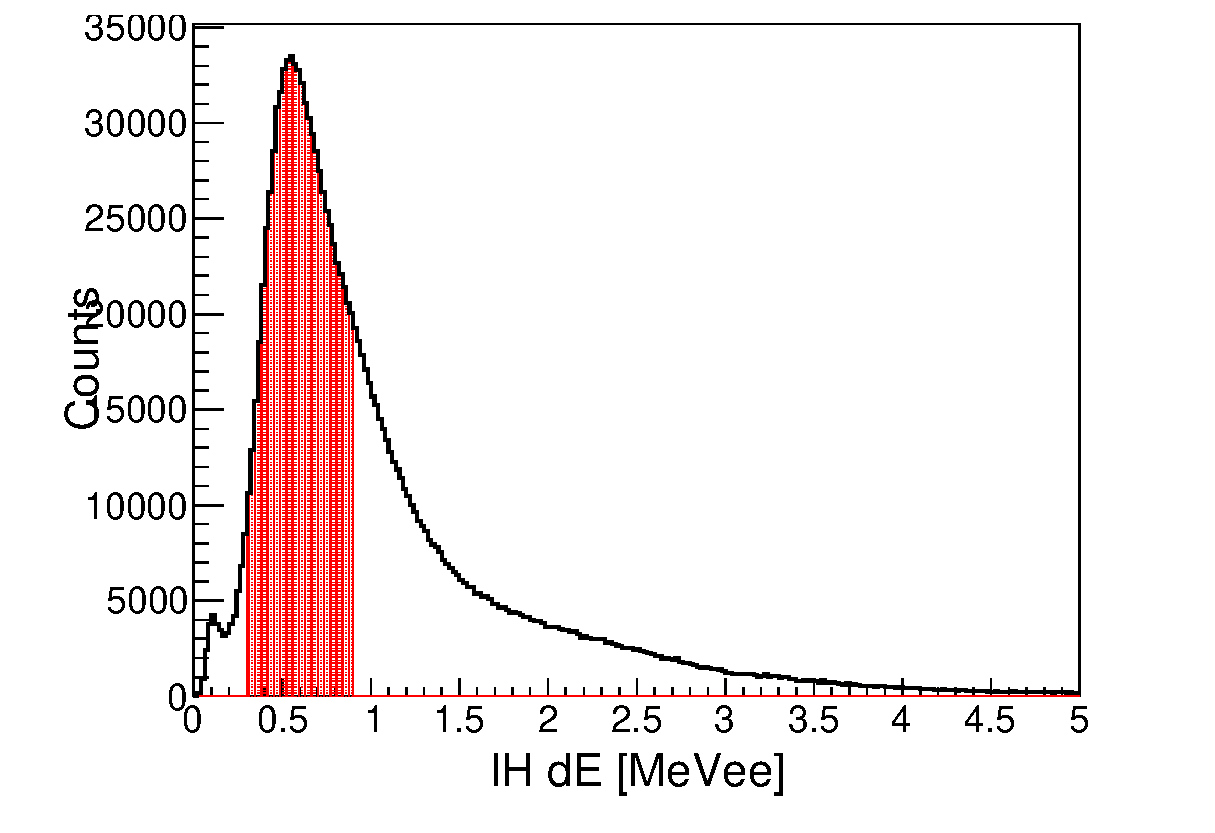
\includegraphics[width=3cm]{../pic/Run68/CDC_eff/IH_dE.eps}
    \end{figure}
  }

  \begin{tabular}{cc}
    \begin{minipage}{0.4\hsize}
      \begin{figure}
        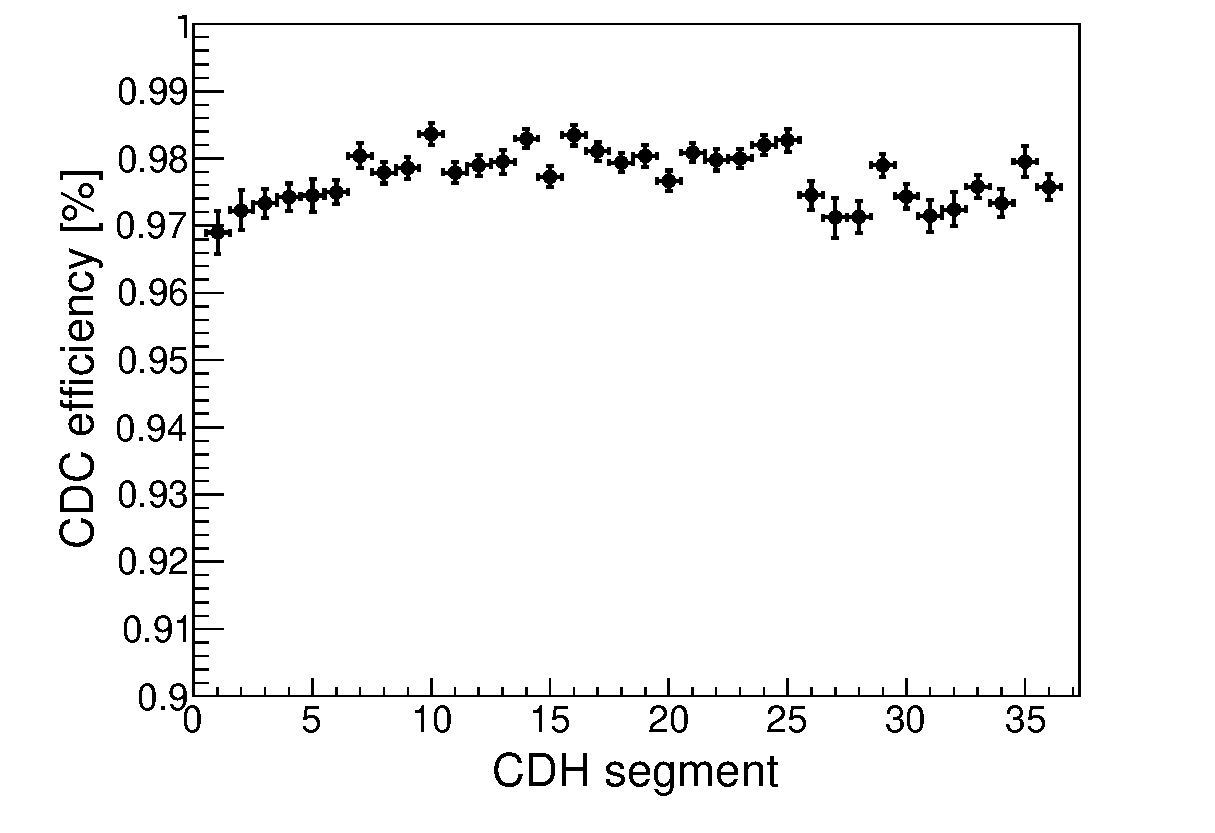
\includegraphics[width=5cm]{../pic/Run68/CDC_eff//CDC_eff_IHCDH.eps}
      \end{figure}
      \vspace{-4mm}
      \centering
      \tiny
      トリガーになったCDHごとのCDC検出効率
        
    \end{minipage}

    \begin{minipage}{0.6\hsize}
      CDHとIHをトリガーとして使う\\
      MIPに近いイベントをとってくるため\\
      CDHとIHのdEは赤枠で選ぶ\\
      T0-CDHのTOFも赤枠で選ぶ\\
      CDHとIHの角度はは45度以内を選ぶ
    \end{minipage}
  \end{tabular}


\end{frame}
